% Circumscribed Parallelepiped
% Author: Axel Pavillet
\documentclass{article}
%%%<
\usepackage{verbatim}
\usepackage{tikz}
\usepackage{tikz-feynman}
\usepackage{adjustbox} % 对齐tikz图用
\usepackage{amsmath,amssymb,amsfonts} % 数学字体
%%%>
\begin{comment}
:Title: Circumscribed Parallelepiped
:Tags: 3D;Geometry;Mathematics
:Author: Axel Pavillet
:Slug: parallelepiped

This is a drawing of a tetrahedron inscibed in a parallelepiped. 
See the following reference p. 58-63 \S 189 to 202

  @BOOK{altshiller1935modern,
    title     = {Modern pure solid geometry},
    publisher = {The Macmillan company},
    year      = {1935},
    author    = {Altshiller-Court, N.},
    address   = {New York},
    edition   = {first},
    lccn      = {35024297},
    url       = {http://books.google.ca/books?id=DDYGAQAAIAAJ}
  }
\end{comment}

\begin{document}

\[
	\begin{aligned}
		%%%%%%%%%%%%%%%%%%%
		% \parbox[c]{2cm}{
      \adjustbox{valign=M}{
			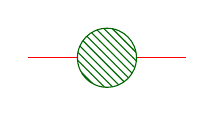
\begin{tikzpicture}[baseline={(current bounding box.center)}]
				\begin{feynman}
					\vertex (a1) at (1,0);
					\vertex[blob,draw=green!40!black, pattern color=green!40!black] (a2) at (2,0){};
					\vertex (a3) at (3,0);
					\diagram* {
					(a1) -- [red] (a2) -- [red] (a3) ,
					};
				\end{feynman}
			\end{tikzpicture}
		}
		%%%%%%%%%%%%%% 
		&=
		%%%%%%%%%%
		\adjustbox{valign=M}{
			\begin{tikzpicture}[baseline={(current bounding box.center)}]
				\begin{feynman}
					\vertex (a1) at (1,0);
					\vertex (a3) at (2,0);
					\diagram* {
					(a1) -- [red] (a3) ,
					};
				\end{feynman}
			\end{tikzpicture}
    }  +
		%%%%%%%%%%%%%%%
		\adjustbox{valign=M}{
			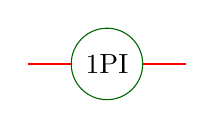
\begin{tikzpicture}[baseline={(current bounding box.center)}]
        \begin{feynman} 
        \vertex (a1) at (1,0); 
        \node[circle,draw=green!40!black, pattern color=green!40!black] (a2) at (2,0){1PI};
        \vertex (a3) at (3,0); 
        \diagram* { 
        (a1) -- [red] (a2) -- [red] (a3) , 
        }; 
        \end{feynman} 
        \end{tikzpicture}
		}+
    %%%%%%%%%%%%%%%%%%%%%%
		\adjustbox{valign=M}{
			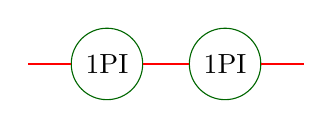
\begin{tikzpicture}[baseline={(current bounding box.center)}]
        \begin{feynman} 
        \vertex (a1) at (1,0); 
        \node[circle,draw=green!40!black, pattern color=green!40!black] (a2) at (2,0){1PI};
        \node[circle,draw=green!40!black, pattern color=green!40!black] (a3) at (3.5,0){1PI};
        \vertex (a4) at (4.5,0); 
        \diagram* { 
        (a1) -- [red] (a2) --[red](a3)--[red](a4),
        }; 
        \end{feynman} 
        \end{tikzpicture}
    }+\cdots \\
    &=\frac{i}{p^2-m^2-M^2(p^2)}
		%%%%%%%%%%%%%%%%%%%%%%
	\end{aligned}
\]

\end{document}


\documentclass{ctexart}
\usepackage{adjustbox}
\usepackage{tikz}

\makeatletter
\newcommand\valignWithTikz[1]{%
  text \tikzcircle{#1} text, $a^2 + \tikzcircle{#1} + b^2$ \par
}
\newcommand\tikzcircle[1]{%
  \tikz[#1] \draw (0, 0) circle (.5);
}

\newcommand\sep{\par\hspace*{10em}}
\makeatother

\begin{document}
\subsection*{默认效果}
绘图底部和文字基线对齐 \sep 
  \valignWithTikz{}

\subsection*{使用 \texttt{baseline} 选项}
\verb|\tikz[baseline=(current bounding box.center)]| \sep
  \valignWithTikz{baseline=(current bounding box.center)}
调整纵向偏移,\verb|\tikz[baseline={([yshift=-.5ex]current bounding box.center)}]| \sep
  \valignWithTikz{baseline={([yshift=-.5ex]current bounding box.center)}}

\subsection*{使用 \texttt{\char`\\adjustbox} 命令的 \texttt{valign} 选项}
\renewcommand{\tikzcircle}[1]{%
  \adjustbox{valign=#1}{\tikz \draw (0, 0) circle (.5);}%
}
\verb|\adjustbox{valign=M}{\tikz ...}| \sep
  \valignWithTikz{M}
\verb|\adjustbox{valign=m}{\tikz ...}| \sep
  \valignWithTikz{m}
\end{document}
